\documentclass{iitthesis}

% Document Options:
%
% Note if you want to save paper when printing drafts,
% replace the above line by
%
%   \documentclass[draft]{iitthesis}
%
% See Help file for more about options.

\usepackage[dvips]{graphicx}    % This package is used for Figures
\usepackage{rotating}           % This package is used for landscape mode.
\usepackage{float}
\usepackage{epsfig}
\usepackage{subfigure}          % These two packages, epsfig and subfigure, are used for creating subplots.
% Packages are explained in the Help document.
\usepackage{colortbl}
\usepackage{booktabs}
\usepackage{mathrsfs}
\usepackage{amsmath, amsthm, amsfonts}
\usepackage[ruled, vlined]{algorithm2e}
\usepackage{cite}

\begin{document}

%%% Declarations for Title Page %%%
\title{Reliable Quasi-Monte Carlo\\
   with Control Variates}
\author{Da Li}
\degree{Master of Science}
\dept{Applied Mathematics}
\date{May 2016}
%\copyrightnoticetrue      % crate copyright page or not
%\coadvisortrue           % add co-advisor. activate it by removing % symbol to add co-advisor
\maketitle                % create title and copyright pages

\prelimpages         % Settings of preliminary pages are done with \prelimpages command

%%%%  Acknowledgement %%%
\begin{acknowledgement}     % acknowledgement environment, this is optional
\par vola
% or \input{acknowledgement.tex} % you need a separate acknowledgement.tex file to include it.
\end{acknowledgement}


% Table of Contents
\tableofcontents
\clearpage

% List of Tables
\listoftables

\clearpage

%List of Figures
\listoffigures

\clearpage

%List of Symbols(optional)
\listofsymbols
\SymbolDefinition{$\mathbb{N}$}{Positive Integers}
\SymbolDefinition{$\mathbb{N}_0$}{Nonnegative Integers}
\SymbolDefinition{$\mathbb{Z}$}{Integers}
\SymbolDefinition{$\mathbb{R}$}{Real numbers}
\SymbolDefinition{$\oplus$}{Digital addition}





%%% Abstract %%%
\begin{abstract}           % abstract environment, this is optional

Recently, Quasi-Monte Carlo (QMC) methods have been implemented in a guaranteed adaptive algorithm. 
This raises the possibility of combining adaptive QMC with efficiency improvement techniques for independent and identically distributed (i.i.d.) Monte Carlo (MC) such as control variates (CV). 

The challenge for adding control variates to QMC is that optimal control variate coefficient for QMC is generally not the same as that for MC. 
Here we propose a method for implementing control variates in a guaranteed adaptive QMC algorithm. 
One merit of using CV with MC is that theoretically the efficiency is always no worse than vanilla MC. 
Our method is implemented in an efficient way so that the extra cost for CV is tolerable.

We test our algorithm on varies problems including option pricing and multivariate normal probability for dimensions from 4 to 64.  
Same tests are performed on adaptive QMC algorithm without CV as a comparision. Our results show that with good CV, the cost of adaptive QMC is greatly reduced compared to vanilla QMC.
 \end{abstract}


\textpages     % Settings of text-pages are done with \textpages command
% Chapters are created with \Chapter{title} command
\Chapter{Introduction}

\Section{The idea}

Recently there are some great results from construction of Quasi Monte Carlo (QMC) methods that can adaptively choose a sample size for given error tolerances\cite{hickernell2014reliable}.   
Our work is trying to combine reliable QMC methods with control variates. We will justify the theory behind it, construct a practical algorithm which can be implemented and tested through high dimensional integration examples.
Control Variates (CV) is a variance reduction technique for IID MC methods.
QMC can be viewed as a deterministic version of IID MC, which outperforms MC for many integrals\cite{avramidis1996integrated}. 
Naturally we wonder if QMC can also benefit from the CV technique. If that is possible, it can be especially useful for problems where we can easily find good control variates.

\Section{The challenge}

The challenge is that for QMC the quadrature points are deterministic instead of random, so the variance minization can not be used. 
Even if one try to use random QMC, the optimal control variate coefficient for QMC is generally not the same as for simple Monte Carlo as explained by Hickernell, Lemieux, and Owen\cite{hickernell2005control}. 
This requires us to figure out a new way to get the optimal coefficients for control variates with Quasi-Monte Carlo.

\Section{Outline}

In chapter 2 we first briefly talk about QMC rule and it's difference between Monte-Carlo. 
Then we introduce control variates and the reliable QMC algorithm that our work is based on. 
In Chapter 3 we show the derivations and theories of our methods along with the corresponding algorithm.
In chapter 4 we demonstrate results from several numerical experiments on option pricing problems. For the final chapter we will discuss the results and possible extensions or improvemnts for the method.
         % Introductory Chapter
\Chapter{Background}

\section{QMC}

\subsection{Digital Sequence}
Talk about the whole idea briefly.
\subsection{QMC}
Introduce QMC.


\section{Control Variates}

\subsection{A Brief Review}
Control variates has been know as variance reduction technique used in Monte Carlo methods.In this part we will brief review some crucial idea of this methods so we can see what's the problem for using it with QMC. \\ 
Suppose we have the following integration approximation problem:
\[I= \int_{[0,1]^d}f(x)dx\]
If we use Monte-Carlo method, the estimator should be: 
\[
\hat{I}(f)=\frac{1}{n}\sum_{i=1}^{n}f(X_i), X_i\sim \mathcal{U}[0,1)^d
\]
Now suppose we have a known function $h$ and its value on the interval
$\int h(x)dx = \theta$.
We construct a new estimator as the following: 
\[ \hat{I}_{cv}(f)=\frac{1}{n}\sum_{i=1}^{n}\Big( f(X_i)-\beta_{mc}(g(X_i)-\theta) \Big) \quad s.t. X_i\sim \mathcal{U}[0,1)\]
We can easily see it's an unbiased estimator.($\mathbb{E}(\hat{I}_{cv}) = I$)\\
Now we want to pick the right $\beta_{mc}$ such that make the estimation more efficient. Base on previous MC error estimating formula~\eqref{}, we know its achievable by minimizing the variance of the estimator, which is: 
\begin{align*}
	\quad &\mathrm{Var}_{mc}(\hat{I}_{cv}) \\
	=& \frac{\mathbb{E}\big([f(X_i)-\beta_{mc}(g(X_i)-\theta)-I]^2 \big)}{n} \\
	=& \frac{\mathbb{E}\big([(f(X_i)-I)^2-2\beta_{mc}(f(X_i)-I)(g(X_i)-\theta)-\beta_{mc}^2(g(X_i)-\theta)^2] \big)}{n}\\
	=& \frac{\mathrm{Var}(f(X_i)-2\beta_{mc}\mathrm{Cov}(f(X_i),g(X_i))+\beta_{mc}^2\mathrm{Var}(g(X_i)) }{n}\\
	=& \frac{\mathrm{Var}(g(X_i)(\beta_{mc}-\frac{\mathrm{Cov}(f(X_i),g(X_i))}{\mathrm{Var}(g(X_i))})^2+\mathrm{Var}(f(X_i)-\frac{\mathrm{Cov}^2(f(X_i),g(X_i))}{\mathrm{Var}(g(X_i))} }{n}
\end{align*}
then the optimal $\beta_{mc}$ is given by: 
$\beta_{mc}=\frac{\mathrm{Cov}(f(X_i),g(X_i))}{\mathrm{Var}(g(X_i))}$\\
In which case the variance become:
\[
\mathrm{Var}_{mc}(\hat{I}_{cv})= \frac{\mathrm{Var}(f(X_i)}{n}[1-\mathrm{corr}^2(f(X_i), g(X_i))]
\]

\subsection{Control Variates with QMC}
Suppose $X_1, \dots, X_n$ are generated by QMC rule, the estimator stays the same.
We can prove it is still unbiased:
\[
\mathbb{E}(\hat{I}_{cv})=\mathbb{E}\Big(\frac{1}{n}\sum_{i=1}^{n}\Big( f(X_i)-\beta(g(X_i)-\theta)\Big)=I 
\]
However, it's not the same case for $\beta_{rqmc}$ since we do not have I.I.D. for $X_i$ this time
\begin{align*}
\mathrm{Var}_{rqmc}(\hat{I}_{cv}) &\not= \frac{\mathbb{E}\big([f(X_i)-\beta_{mc}(g(X_i)-\theta)-I]^2 \big)}{n}\\
&=\mathrm{Var}_{rqmc}\Big( \hat{I}- \beta_{rqmc}\hat{G}\Big)\quad , \hat{G}=\sum_{i=1}^{n}(g(X_i)-\theta)\\
\beta_{rqmc}^*&= \mathrm{Var} (\hat{G})^{-1}\mathrm{Cov} (\hat{G}, \hat{I})
\end{align*}

\section{Reliable Adaptive QMC with digital sequence}
\subsection{Idea of adaptive cubature algorithm}
One practical problem for QMC method is that how to get the sample size big enough for a required error tolerance. 
The idea in work of Hickernell and Jiménez Rugama(2014) is to construct a 
QMC algorithm with reliable error estimation on digital sequence. 
Here we briefly summarize their results.
The error of QMC method on digital sequence can be expressed in terms of Walsh coefficients of the integrand on certain cone conditions. 
\begin{align*}
&\Big|\int_{[0,1)^d}f(x)dx - \hat{I}_m(f)\Big| \leq a(r,m) \sum_{\lfloor 2^{m-r-1} \rfloor}^{2^{m-r}-1} |\hat{f}_{m,k}|\\
&\hat{I}_m(f): = \frac{1}{b^m}\sum_{i=0}^{b^m-1}f(z_i\oplus \Delta)\\
&\hat{f}_{m,k}=\text{ discrete Fourier coefficients of }f\\
&a(r,m) =\text{ inflation factor that depends on } \mathcal{C}
\end{align*}
Here is the cone condition.
\begin{align*}
	&\Big|\int_{[0,1)^d}f(x)dx - \hat{I}_m(f)\Big|
    \leq \sum {\bigcirc} 
	\leq \sum {\Box}
	\leq a(r,m) \sum_{\lfloor b^{m-r-1} \rfloor}^{b^{m-r}-1}|\hat{f}_{m,k}|\\
    &\bigcirc:= \sum_{\lambda=1}^{\infty}| \hat{f}_{\lambda b^m}|,\quad  
    \Box:= \sum_{\kappa=b^{l-1}}^{b^l-1}|\hat{f}_\kappa|,\quad
    \Diamond:=\sum_{\kappa=b^m}^{\infty}|\hat{f}_{\kappa}|\\
    &\mathcal{C}:=\Big\{\sum{\bigcirc} \leq \sum{\Diamond} \leq \sum{\Box}\Big\}
\end{align*}

\includegraphics[width=0.8\textwidth]{figures/cone.bmp}
         % Chapter 2
\Chapter{Reliable adaptive QMC with CV}

\Section{Idea to add control variates to reliable adaptive QMC}

The whole method starts with an idea similar to traditional control variates technique for MC.
If we know the integration of a function $\boldsymbol{h}=(h_1,\dots,h_J)$ on the interval same as our $f$, say $\int_{[0,1)^d}h_jdx=\theta_j$, then we can define a new function $g$:
\begin{align}\label{eq:defg}
    & g:=f-(\boldsymbol{h}-\boldsymbol{\theta})\boldsymbol{\beta}\\
    \notag
    &\text{s.t. }\boldsymbol{\theta}=(\theta_1,\dots,\theta_J),
    \boldsymbol{\beta}=(\beta_1,\dots,\beta_J)^T.
\end{align}
Then easily we can find that if we replace $f$ with $g$, the integration stays the same:
\[
	\int_{[0,1)^d}gdx
        =\int_{[0,1)^d}f-(\boldsymbol{h}-\boldsymbol{\theta})\boldsymbol{\beta}dx
			=\int_{[0,1)^d}fdx.
\]
Now we wonder if one can still use the same method as MC, the answer is no and the reason is in the next section. 

\Section{The problem of CV with random QMC}

The problem is that QMC is not a random process and we simply can't use the minimizing mean squre error trick as shown earlier anymore. However, one can use random QMC instead to `restore' the randomness to QMC \cite{}. 
Random QMC use a different way for generating $X_i$, they are still identical(i.e.\ from same distribution) but not independent, which will make it different from CV with MC.

Suppose $X_1, \dots, X_n$ are generated by QMC rule, the estimator stays the same
\[
    \hat{I}_{cv}(f)=\frac{1}{n}\sum_{i=1}^{n}\Big[ f(X_i)-\beta_{qmc}[h(X_i)-\theta] \Big] \quad X_i\in \mathcal{U}(0,1)
\]
We can easily prove it is still unbiased
\[
\mathbb{E}(\hat{I}_{cv})=\mathbb{E}\Big(\frac{1}{n}\sum_{i=1}^{n}\Big[f(X_i)-\beta_{mc}[h(X_i)-\theta] \Big] \Big)=I 
\]
However, it's not the same case as MC like we presented before, because we do not have i.i.d for $X_i$ this time
\[
\mathrm{Var}_{qmc}(\hat{I}_{cv}) \not=\frac{1}{n}\mathrm{Var}\Big(f(X_i)-\beta_{mc}[h(X_i)-\theta]\Big)\\
\]
Instead the variance become
\begin{align*}
    \mathrm{Var}\hat{I}_{cv})  
    &=\mathrm{Var}\Big( \hat{I}- \beta_{qmc}\hat{H}\Big)
    \quad s.t.\; \hat{I}=\sum_{i=1}^{n}f(X_i),\; \hat{H}=\sum_{i=1}^{n}[h(X_i)-\theta]\\
    &=\mathrm{Var}(\hat{I})-2\beta_{qmc}\mathrm{Cov}(\hat{I},\hat{H})+\beta_{qmc}^2\mathrm{Var}(\hat{H})\\
    &=\mathrm{Var}(\hat{H})\Big(\beta_{qmc}-\frac{\mathrm{Cov}(\hat{I},\hat{H})}{\mathrm{Var}(\hat{H})}\Big)^2+\mathrm{Var}(\hat{I})-\frac{\mathrm{Cov}(\hat{I},\hat{H})}{\mathrm{Var}(\hat{H})}
\end{align*}
The optimal $\beta_{qmc}$ is
\begin{equation}
    \beta_{qmc}^*= \mathrm{Var} (\hat{H})^{-1}\mathrm{Cov} (\hat{I}, \hat{H})
    \label{eq:optBetaqmc}
\end{equation}
which leave the variance to be
\[
    \mathrm{Var}_{qmc}(\hat{I}_{cv})=\mathrm{Var}(\hat{I})\big(1-\mathrm{corr}^2[\hat{I}, \hat{H}]\big)
\]

Now we are interested that if our previous formula for $\hat{\beta}_{mc}$ could be an estimation for $\hat{\beta}_{qmc}$. The fact is that they are generally not the same. Let's take the covariance part of formula ~\eqref{eq:optBetaqmc} and ~\eqref{eq:optBeta} to see the difference. 
\begin{align*}
    \mathrm{Cov}(\hat{I}, \hat{H})=&\int [f(X_1)+\dots+f(X_n)][h(X_1)+\dots+h(X_n)]\; d\mathbf{X}\\
    =&\int [\sum_{i=1}^{n}f(X_i)h(X_i) + \sum_{i,j=1}^{i\neq j}f(X_i)h(X_j)]\; d\mathbf{X}\\
    \neq&\int f(X_i)h(X_i)dX_i\\
    =&\mathrm{Cov}x[(f(X_i),h(X_i)]
\end{align*}
There is also a very good example from Hicknell and Lemieux(2005)\cite{hickernell2005control}'s paper, showing that $\beta_{mc}$ and $\beta_{qmc}$ can make a quite different results in some cases. 


\Section{A new way to find $\beta$} 

As we stated in previous section, we can not find optimal $\beta$ by minimizing variance of estimator like Monte-Carlo. 
However, if using the guaranteed adaptive QMC method introduced in chapter 2, we may have another way to find $\beta$.

Recall equation~\eqref{eq:errBound} the error bound for new estimator of $g$ still holds
\begin{equation}\label{eq:qmccvErr}
	\Big|\int_{[0,1)^d}gdx - \hat{I}_m(g)\Big| \leq a(r,m) \sum_{\lfloor 2^{m-r-1} \rfloor}^{2^{m-r}-1} |\tilde{g}_{m,k}|
\end{equation}
Naturally, the new estimator become
\begin{equation}\label{eq:estcv}
    \hat{I}_m({g}): = \frac{1}{b^m}\sum_{i=0}^{b^m-1}g(z_i+\Delta)
\end{equation}


From~\eqref{eq:qmccvErr} it is clear that the optimal $\beta$ is the one that minimize the error term. 
\begin{align}
    \label{eq:optbeta1}
    \boldsymbol{\beta}^*
    &=\min_{\boldsymbol{\beta}}\sum_{\kappa=b^{m-r-1}}^{b^{m-r}-1} |\hat{g}_{\kappa}|\\
    \label{eq:optbeta2}
    &=\min_{\boldsymbol{\beta}}\sum_{\kappa=b^{m-r-1}}^{b^{m-r}-1}|\hat{f}_\kappa
    -(\hat{\boldsymbol{h}}_\kappa - \hat{\boldsymbol{\theta}})\boldsymbol{\boldsymbol{\beta}}|
    && \hat{\boldsymbol{h}}_\kappa=(\hat{h}_{\kappa,1},\dots, \hat{h}_{\kappa,J}),
    \hat{\boldsymbol{\theta}}=(\hat{\theta}_{\kappa,1},\dots,\hat{\theta}_{\kappa,J})\\
    \label{eq:optbeta3}
    &=\min_{\boldsymbol{\beta}}\|\hat{\boldsymbol{f}}-\hat{\boldsymbol{H}}\boldsymbol{\beta}\|_1
    && \hat{\boldsymbol{f}}= (\hat{f}_{b^{m-r-1}},\dots,\hat{f}_{b^{m-r}-1)})^T \\
    \label{eq:optbeta4}
    &\approx\min_{\boldsymbol{\beta}}\|\hat{\boldsymbol{f}}-\hat{\boldsymbol{H}}\boldsymbol{\beta}\|_2
    && \hat{\boldsymbol{H}}= (\hat{\boldsymbol{H}}_1, \dots, \hat{\boldsymbol{H}}_J)\\
    & \notag 
    &&\hat{\boldsymbol{H}_j}=(\hat{h}_{b^{m-r-1},j}-\hat{\theta}_j,\dots, \hat{h}_{b^{m-r}-1,j}-\hat{\theta}_j)^T
\end{align}

The second equivalence is not hard to get, but the third one may not be so obvious. Let's consider it backwards. Suppose we have a vector A and it's $\mathcal{L}_1$-norm.
\[
   A=
    \begin{pmatrix}
        f_1-z_1\\
        f_2-z_2\\
        \hdots\\
        f_n-z_n
    \end{pmatrix},\quad
    \|A\|_1=\sum_{i=1}^{n}|f_i-z_i|, \quad
    z_i:=(\boldsymbol{h}_i-\boldsymbol{\theta})
\]

If we replace the index,$A$ is exactly what's inside the $\mathcal{L}_1$-norm in ~\eqref{eq:optbeta3}. 
Hence we justified the third equivalence. The reason we use an approximation instead, i.e. the $\mathcal{L}_1$-norm, is because there is no efficient way to solve it compared to existing least square methods.

\Section{The problem with $\theta$}

We noticed a problem in solution for optimal $\beta$, which is we do a lot of subtractions with $\theta$. This could be a large cost when we have difficult functions which means $b^{m-r}$ could be very large number. Therefore we present a way to avoid that part.

The idea is form a observation that Walsh transform of $\theta$ in~\eqref{qe:optbeta2} is actually zero, since $\hat{h}_\theta= \theta\delta_{\kappa,0}$ and the summation is not start from $\kappa=0$.

This simplifies~\eqref{eq:optbeta2} to the following. Note that we only need the information of function $f$ and $h$ to calculate $\beta^*$, $\theta$ has been get rid of the optimization process.
\begin{align}
    \boldsymbol{\beta}^*
    \label{eq:optbetanew}
    &=\min_{\boldsymbol{\beta}}\sum_{\kappa=b^{m-r-1}}^{b^{m-r}-1}|\hat{f}_\kappa
    -(\hat{\boldsymbol{h}}_\kappa - \hat{\boldsymbol{\theta}})\boldsymbol{\boldsymbol{\beta}}|\\
    &=\min_{\boldsymbol{\beta}}\sum_{\kappa=b^{m-r-1}}^{b^{m-r}-1}|\hat{f}_\kappa
    -(\hat{\boldsymbol{h}}_\kappa - \boldsymbol{\theta}\delta_{\kappa,0})\boldsymbol{\boldsymbol{\beta}}| \notag \\
    &=\min_{\boldsymbol{\beta}}\sum_{\kappa=b^{m-r-1}}^{b^{m-r}-1}|\hat{f}_\kappa
    -\hat{\boldsymbol{h}}_\kappa \boldsymbol{\boldsymbol{\beta}}|
    && \hat{\boldsymbol{f}}= (\hat{f}_{b^{m-r-1}},\dots,\hat{f}_{b^{m-r}-1)})^T \notag\\
    &=\min_{\boldsymbol{\beta}}\|\hat{\boldsymbol{f}}-\hat{\boldsymbol{H}}\boldsymbol{\beta}\|_1
    && \hat{\boldsymbol{H}}= (\hat{\boldsymbol{H}}_1, \dots, \hat{\boldsymbol{H}}_J)\notag \\
    &\approx\min_{\boldsymbol{\beta}}\|\hat{\boldsymbol{f}}-\hat{\boldsymbol{H}}\boldsymbol{\beta}\|_2
    &&\hat{\boldsymbol{H}_j}=(\hat{h}_{b^{m-r-1},j},\dots, \hat{h}_{b^{m-r}-1,j})^T \notag
\end{align}

The same problem happened with the estimator~\eqref{eq:estcv}. We have the similar solution for that.
\begin{align}
    \notag
    \hat{I}_m({g})
    & = \frac{1}{b^m}\sum_{i=0}^{b^m-1}g(z_i+\Delta)\\
    \notag
    & = \frac{1}{b^m}\sum_{i=0}^{b^m-1}f(z_i+\Delta)-(\boldsymbol{h}(z_i+\Delta)-\boldsymbol{\theta})\boldsymbol{\beta}\\
    \label{eq:estcvnew}
    & = \frac{1}{b^m}\sum_{i=0}^{b^m-1}[f(z_i+\Delta)-\boldsymbol{h}(z_i+\Delta)\boldsymbol{\beta}]+\boldsymbol{\theta}\boldsymbol{\beta}
\end{align}

After organize it the in format of~\eqref{eq:estcvnew}, $\theta$ is eliminated from the summation part. From these two parts of work on $\theta$ we managed to save $\frac{b-1}{b}b^{m-r}+b^m$ operations of subtraction.


\Section{The modified method}

Now we make the following changes 
\begin{align*}
    g&=f-\beta h\\ 
    \hat{I}_m({g})&= \frac{1}{b^m}\sum_{i=0}^{b^m-1}g(z_i+\Delta)
\end{align*}

And we have the following equivalence 
\begin{align*}
    \int_{[0,1)^d}fdx &= \int_{[0,1)^d}gdx +\theta\beta\\ 
    \hat{I}_m(f) &= \hat{I}_m(g)+\theta\beta
\end{align*}

So the estimation error becomes 
\[
\Big| \int_{[0,1)^d}fdx- \hat{I}_m(f) \Big|
    =\Big| \int_{[0,1)^d}gdx- \hat{I}_m(g) \Big|
\]

Here if our $g$ is in the cone we introduced earlier~\eqref{eq:cone}, then we can use the results from Hickernell and Jiménez Rugama(2014)\cite{hickernell2014reliable}, the error is bounded by
\[
\Big|\int_{[0,1)^d}gdx - \hat{I}_m(g)\Big| \leq a(r,m) \sum_{\lfloor 2^{m-r-1} \rfloor}^{2^{m-r}-1} |\tilde{g}_{m,k}|
\]
This leads to the same algorithm suggested by Hickernell and Jiménez Rugama(2014)\cite{hickernell2014reliable}, but since we are using control variates, several modifications have to be made.

\Section{The Algorithm}

We now give the algorithm for reliable adaptive QMC with control variates 
using digital sequence.
\begin{algorithm}[h]
\DontPrintSemicolon
\KwData{function $f$ and $\boldsymbol{H}$; 
    value of $\int_{[0,1)^d}h_jdx=\theta_j$; tolerance $\varepsilon$} 
    \KwResult{$\hat{I}(f)$; samples size; optimal $\beta$}
\Begin{
    \nl $m, r=$ start numbers, $x=$ $2^m$ sobolset points\;
    \nl \label{alg:alg1kappaFWT}
    get kappa map($\tilde{\kappa}$) and Walsh coefficients($\tilde{f},\tilde{\boldsymbol{H}})$ using algorithm~\ref{alg:kappaFWT} \;
    \nl \label{alg:alg1beta}
    $\boldsymbol{\beta}=
    \tilde{H}\big\{ \tilde{\kappa}[x(a:b)]\big\}\backslash
    \tilde{f}\big\{ \tilde{\kappa}[x(a:b)]\big\}, (a:b)=(2^{m-r-1}:2^{m-r}-1)$\;
    \nl 
    $g= f-\boldsymbol{H}\boldsymbol{\beta}$, repeat step~\ref{alg:alg1kappaFWT} on $g$\;
    \nl \label{alg:alg1stilde}
    $\tilde{S}_{m-r,m}(g)= \sum_{a}^{b}
    \Big| \tilde{g}\big\{ \tilde{\kappa}[x(a:b)]\big\}\Big|$ \;
    \nl \label{alg:alg1cone} 
    check whether $g$ is in the cone\;
    \nl \label{alg:alg1exit}     
    \If{$a(m,r)\tilde{S}_{m-r,m}(g)\leq \varepsilon$}
    {return $\hat{I}_m(g)=\sum_{i=0}^{2^m-1}f[x(i)]+\boldsymbol{\theta}\boldsymbol{\beta}$\;
    return $\boldsymbol{\beta},n=2^m$}
    \nl
    \For{$m=m+1:mmax$}
    {$xnext=$ next $2^{m-1}$ sobolset points\;    
        repeat step~\ref{alg:alg1kappaFWT} on $[x,xnext]$\;
        repeat step~\ref{alg:alg1stilde}, ~\ref{alg:alg1cone}, ~\ref{alg:alg1exit}\;
        }
    }
\caption{Reliable Adaptive QMC with control variates}\label{alg:qmccv}
\end{algorithm}

Note that for generating kappa map, i.e. step~\ref{alg:alg1kappa}in Algorithm~\ref{alg:qmccv}, we used an explicit way to generate it.   

Another importent point need to be mentioned is that in our algorithm, we used an iterative way, which may require recalculating $beta$ each time m increment.

\begin{algorithm}
\DontPrintSemicolon
\KwData{function $f$; $\mathit{Y}_v^{(m)}$ ; $m \in \mathbb{N}_0$} 
    \KwResult{$\tilde{\kappa}$; $\tilde{S}_{m-r,m}(f)$}
\Begin{
    \If{$m=0$}
    {$\mathring{\mathbf{v}}(0) = 0$}
    \If{$m\geq1$}{\For{$m:1:-1$}{$\mathring{\mathbf{v}}_m(\mathbf{k})=\mathring{\mathbf{v}}_m-1(\mathbf{k})$\; $\mathring{\mathbf{v}}_m(\mathbf{k})=\mathbf{k},\; \mathbf{k}=b^{m-1}, \dots, b^m-1$}}
    \For{$l=m-1:max(1,m-r):-1$}
    {\For{$k=1:b^l-1$}
        {$\forall a \in \mathbb{F}_b$, find $a$ s.t. $|\mathit{Y}^{(m)}_{\mathring{\mathbf{v}}(k+a^*b^l)}| \geq |\mathit{Y}^{(m)}_{\mathring{\mathbf{v}}(k+ab^l)}|$}
    }
}
\caption{kappa map and discrete Walsh coeffcients}\label{alg:kappaFWT}
\end{algorithm}
\iffalse
\Section{When beta is not accurate?}

Note that in algorthm~\ref{alg:qmccv}, we didn't recalculate $\beta$ for every iteration. The reason is that for most functions this is not neccesary, but in certain case $\beta$ need to be updated to get the right answer. Here is an example showing that for certain strange functions beta needs to be updated. 

\fi
         % Chapter 3
\Chapter{Numerical Experiment}
\section{When beta is not accurate?}
Examples to show for certain functions beta needs to be updated. 
\section{Option Pricing}
Option Pricing has always been a challenging topic in financial mathematics.
Add some reasons?\\
Hence it became a good application for our QMC algorithm.
Here we are going to demonstrate several examples of pricing different options with ccontrol variates.

\subsection{Asian Option}
There are two types of asian options, depends on which types of mean you want to use.For this example we take arithematic mean asian call option as our target function, whose payoff function is:
\[ C_{T}^{Amean} = \max\Big(\frac{1}{d}\sum_{j=1}^{d}S(jT/d)-K, 0\Big)\]
\begin{table}[H]
    \centering
	\begin{tabular}{lllllll}
		\toprule
		 S0 & K & TimeVector & r & volatility & abstol & reltol \\
		\midrule
		 120  & 130 & 1/52:1/52:16/52 & 0.01 & 0.5 & 1e-3 & 0\\ 
		\bottomrule
	\end{tabular}
	\caption{Parameter Setup for Up and In Barrier Call Option}
\end{table}
\begin{table}[H]
    \centering
	\begin{tabular}{  
		r>{\columncolor[gray]{.8}} r >{\color{white}\columncolor[gray]{.2}}r 
		r>{\columncolor[gray]{.8}} r >{\color{white}\columncolor[gray]{.2}}r} 
	\toprule
	\multicolumn{3}{c}{Sample Size}
		&\multicolumn{3}{c}{Time Cost} \\
	\cmidrule(r){1-6}
	 cubSobol&cv\_old&cv\_new
	 &cubSobol&cv\_old&cv\_new\\
        \midrule
		 65535&8192&9011
		&0.2783&0.1034&0.0673\\
	\bottomrule
	\end{tabular}
	\caption{Results of cubSobol, cv\_old and cv\_new with Asian Option}
\end{table}
Figure~\ref{} shows decrease rate the walsh coefficients for the target function and control variates in this example. 
\begin{figure}[H]
    \caption{}
    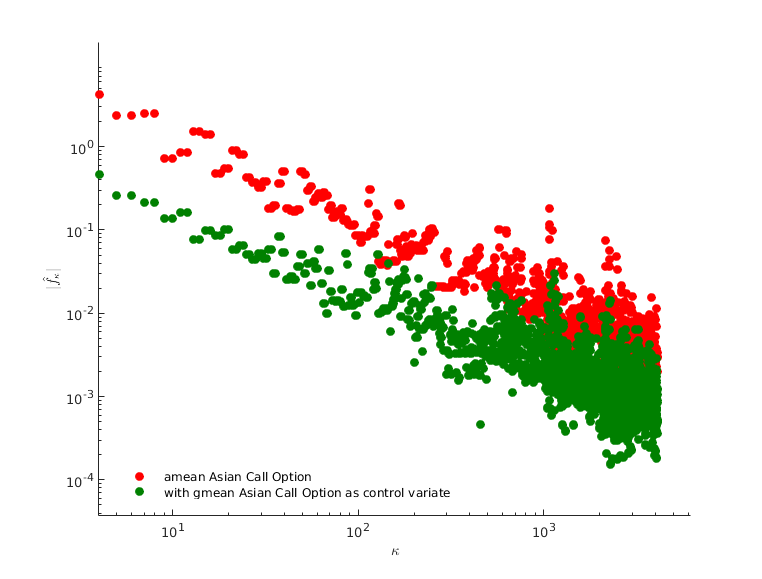
\includegraphics[width=0.8\textwidth]{figures/cvEx1.eps}
\end{figure}

\subsection{Barrier Option}
We will take up and in barrier call option as an example.
Here is the payoff function for up and in barrier call option.
\[ C_{T}^{U\&I} = (S_T-K)^+1_{ \{\max S_t \geq Barrier\}} \]
From the payoff function it is naturally to consider european call option as 
control variates. Since if we take the barrier same as strike price, then this is just an european call option.  
Table~\ref{BarrierPara} shows our setup for the barrier option.
\begin{table}[H]
    \centering
	\begin{tabular}{lllllll}
		\toprule
		 S0 & K & TimeVector & r & volatility & abstol & reltol \\
		\midrule
		 120  & 130 & 1/52:1/52:16/52 & 0.01 & 0.5 & 1e-3 & 0\\ 
		\bottomrule
	\end{tabular}
	\caption{Parameter Setup for Up and In Barrier Call Option}
    \label{tb:BarrierPara}
\end{table}
\begin{table}[H]
    \centering
	\begin{tabular}{l
		r>{\columncolor[gray]{.8}} r >{\color{white}\columncolor[gray]{.2}}r 
		r>{\columncolor[gray]{.8}} r >{\color{white}\columncolor[gray]{.2}}r} 
	\toprule
	Barrier &\multicolumn{3}{c}{Sample Size}
		&\multicolumn{3}{c}{Time Cost} \\
	\cmidrule(r){2-7}
	 &cubSobol&cv\_old&cv\_new
	 &cubSobol&cv\_old&cv\_new\\
        \midrule
	140  & 524288&78643& 65535
	     & 1.874& 0.5016&0.2743 \\ 
	135  & 524288& 5802&6963
	     & 1.959& 0.0781&0.0519 \\ 
	130  & 524288& 1024&1024
	     & 1.876& 0.0270 & 0.0199 \\
	\bottomrule
	\end{tabular}
	\caption{Results of cubSobol, cv\_old and cv\_new with Barrier Option}
\end{table}
We then took three different barrier as listed in table~\ref{tb:BarrierResults},
then we compared both oringinal cubSobol algorithm and the one with our modification as described in Chapter 4. \\
We can see from the results in table~\ref{tb:BarrierResults}

         % Chapter 4
\Chapter{Conclusion}

\Section{Discussion}

So far there are only few QMC algorithms that can adaptively determine the sample size needed based on integrand values. 
This is because the estimation of error for QMC is hard. 
Studies show that if using quasi-standard error there will be some serious drawbacks\cite{owen2006warnock}. 
There is also a way using internal replications of IID randomized QMC rules, but the number of replications are not known\cite{hickernell2005control}.

For CV with QMC the research progress is also limited since it is hard to estimate the value of CV coefficients as we stated in chapter 3. 
Hickernell and Jim{\'e}nez Rugama (2014) \cite{hickernell2014reliable}'s work on building a QMC method provides a reliable and adaptive way to use QMC, as well as 
gives us insights into combining reliable adaptive QMC with CV.    
The main idea of the reliable adaptive QMC is to bound the error of estimation using summation of partial Walsh coefficients. 
We utilize the same idea for calculating the optimal coefficient for CV.  
In order to compensate the extra computation cost for CV, we used several techniques in our design to keep those cost minimal.

We test our algorithm on several option pricing problems under Black-Scholes scheme. We find the accuracy of algorithm is consistent and reliable. 
Comparison of QMC with CV and normal QMC is performed on different pairs of options, the results show that using the proper CV we can make improvements over vanilla QMC methods. 
We also provide an example of computing multivariate normal probability using CV with estimated mean. It is shown in certain cases multiple CV outperforms single CV.       

\newpage

\Section{Future work}

There are several unsolved problems in our work, of which we have not found the answers yet. 
To start with, we use the least square regression solution to approximate the least absolute error regression for CV coefficients. 
Is there a way to do $\mathcal{L}_1$ regression more efficiently? Can it offer enough improvement on computational cost to compensate its own cost?    
This leads to the second problem. In our numerical examples we do not update CV coefficients in each iteration. 
The reason is that we find doing this updating requires a lot of recalculations of previous terms, which could reduce the advantage brought by CV. For further research we hope to find a way to update $\beta$ more efficiently.      
Another possible work for future research is that we can extend this method to rank-1 lattices\cite{rugama2014adaptive}. 
The idea for getting CV coefficients is the same, but due to the different points structure compared to digital sequences, some effort has to be done for adaption of the method.  
         % Chapter 4

%\include{appendixA}
%\include{appendixB}

\clearpage

\bibliography{ref}{}
\bibliographystyle{ieeetr}

\end{document}  % end of document
